\let\textcircled=\pgftextcircled
\chapter{Project Outline}
\label{chap:proj_outline}

\section{Description of tasks}

\begin{itemize}
    \item \textbf{Project environment setup}
    \item \textbf{Review of related research}
    \item \textbf{CNN implementation}
    \item \textbf{Testing and debugging}
    \item \textbf{Training of CNN}
    \item \textbf{Parameter tuning}
    \item \textbf{Evaluation}
    \item \textbf{Validation with different datasets}
\end{itemize}



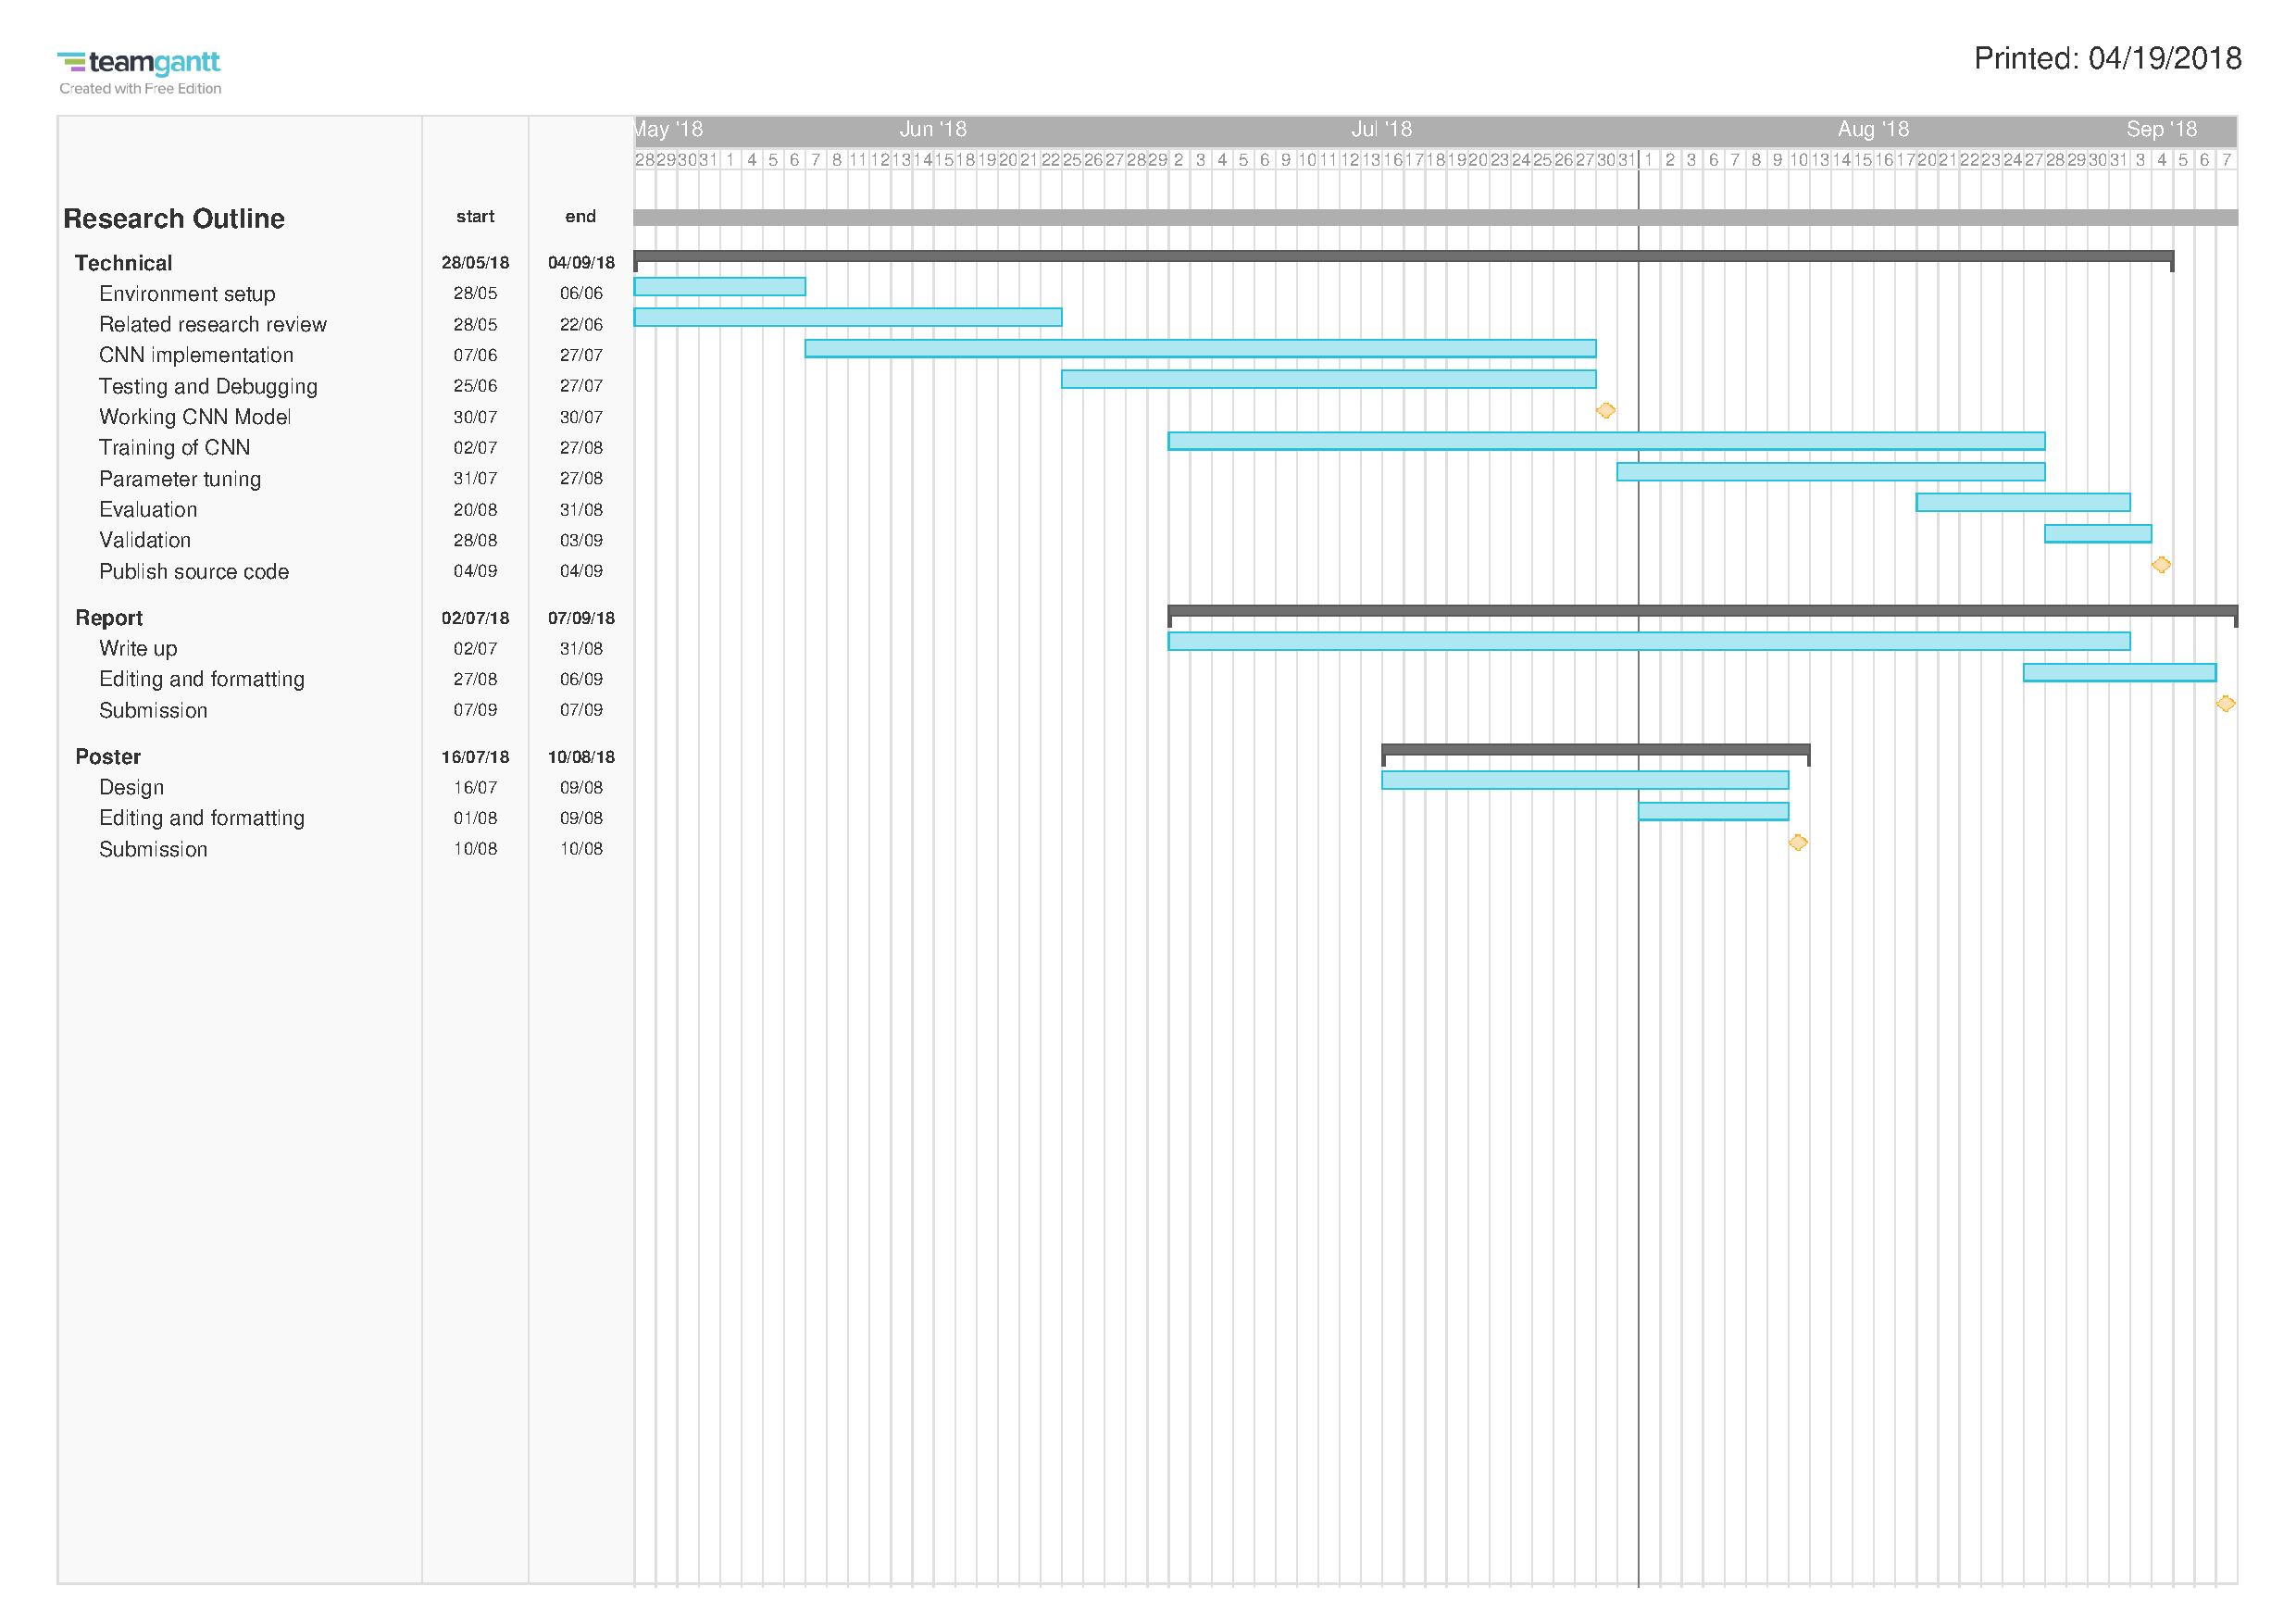
\includepdf[pages=-]{outline.pdf}


\section{Risk Analysis}
 
\subsection*{Technology incompatibility}

\subsection*{Unrealistic timeline}
	
	
	
\subsection*{Poor evaluation results}



\subsection*{Altered requirements}


\subsection*{Overestimated capabilities}


\subsection*{Illness}


\subsection*{Data loss}




\begin{center}
    \begin{tabular}{ | l | l | l | p{5cm} |}
    \hline
    Risk Factor & Risk Rank & Contributors & Mitigation and Contingencies \\ \hline
    Technology incompatibility & High & Cutting edge software & \\ \hline 
    Unrealistic timeline & High & & \\ \hline
    Poor evaluation results & Medium & & \\ \hline
    Altered requirements & Medium & & \\ \hline
    Overestimated capabilities & High & & \\ \hline
    Illness & Medium & & \\ \hline 
    Data loss & Low &  & Frequent pushing to Github repository\\ \hline 

   
    \hline
    \end{tabular}
\end{center}





